\RequirePackage[]{silence}
\WarningFilter{latex}{Marginpar on page}
\WarningFilter{lcg}{Using an already existing counter rand}
\documentclass[article]{aaltoseries}
\usepackage[utf8]{inputenc}
\usepackage[english]{babel}
\usepackage{IEEEtrantools}
\usepackage[hyphens]{url} % allow hyphens to break urls
\Urlmuskip=0mu  plus 1mu % allow for some spacing inside urls
\usepackage[hidelinks]{hyperref}
\usepackage[acronym]{glossaries}
\usepackage{amsfonts}
\usepackage{todonotes}
\usepackage[normalem]{ulem}
\usepackage{xcolor}
\usepackage{xspace}
\usepackage{textcomp}
\usepackage{etoolbox}
\usepackage{enumitem}
\usepackage[numbers]{natbib}
\newcommand{\TODO}[1]{\todo[inline]{#1}}
\newcommand{\jwnote}[1]{\todo[size=\small,color=blue!40]{#1}}
\newcommand{\JWNOTE}[1]{\todo[size=\small,inline,color=blue!40]{#1}}
\newcommand{\modif}[1]{\textcolor{blue}{#1}}
\newcommand\remove{\bgroup\markoverwith
{\textcolor{red}{\rule[0.5ex]{2pt}{0.8pt}}}\ULon}
\newcommand{\discuss}[1]{\todo[size=\small,color=green!40]{#1}}

% \geometry{left=4cm,right=4cm,marginparwidth=3.5cm,marginparsep=5mm} % TODO: remove
% \geometry{left=1cm,right=7cm,marginparwidth=6.5cm,marginparsep=5mm} % TODO: remove
% \reversemarginpar % for todo notes on the wider side
% \geometry{marginparwidth=5cm,marginparsep=3mm} % TODO: remove

% Use “\tocite{}” to get “citation needed” in document
% \newcommand\tocite[1]{
% 	\todo{\ifstrempty{#1}{Citation needed}{#1}}
% 	[\,\textbf{\color{red}!}\,]
% }


% ************************ Custom Referencing **********************************
\newcommand{\Fref}[1]{Figure~\ref{#1}}
\newcommand{\fref}[1]{figure~\ref{#1}}
\newcommand{\Tref}[1]{Table~\ref{#1}}
\newcommand{\tref}[1]{table~\ref{#1}}
\newcommand{\Eref}[1]{Equation~\ref{#1}}
\newcommand{\eref}[1]{equation~\ref{#1}}
\newcommand{\Sref}[1]{Section~\ref{#1}}
\newcommand{\sref}[1]{section~\ref{#1}}
\newcommand{\Lref}[1]{Listing~\ref{#1}}
\newcommand{\lref}[1]{listing~\ref{#1}}


\newcommand{\app}[1]{A\textsc{pp}$_{#1}$\xspace}

\glsenableentrycount
\renewcommand\gls\cgls
\renewcommand\glspl\cglspl
\renewcommand\Gls\cGls
\renewcommand\Glspl\cGlspl
\newacronym{os}{OS}{operating system}
\newacronym{vm}{VM}{virtual machine}

\title{Android App Collusion}


\author{Ervin Oro% Your first and last name: do _not_ add your student number
\\\textnormal{\texttt{ervin.oro@aalto.fi}}} % Your Aalto e-mail address
\affiliation{\textbf{Tutor}: Jorden Whitefield} % First and last name of your tutor

%==========================================================

\begin{document}
\bstctlcite{BSTcontrol}

\maketitle
% \todo{set proper margins and document format}
%==========================================================

\begin{abstract}

As people increasingly rely on their smartphones, both the number and complexity of malware attacks against Android are growing. While defending Android is an active area of research, a number of threats, e.g., app collusion, cannot yet be reliably detected nor defended against. App collusion is a secret collaboration between apps with malicious intentions. This report surveyed state-of-the-art literature discussing methods that can be used for collusion on Android, and known examples of such collusion. It also reviewed existing approaches to app collusion detection, and their limitations. Existing literature was determined to have significant limitations, such as outdated or uncredible claims and inconsistent definitions. Further research is required to develop feasible protections against Android app collusion, and the unified definition and criteria proposed in this report could be developed into a common framework for assisting the research community in achieveving that goal.

\vspace{3mm}
\noindent KEYWORDS: Collusion, Android security, Mobile security

\end{abstract}

%============================================================

\section{Introduction}
\label{sec:intro}

Android is an \gls{os} that is primarily designed for mobile devices, e.g., smartphones and tablets. With more than two billion active devices~\cite{AOSP2018}, it is estimated to be the most widely used \gls{os}, surpassing even Microsoft Windows~\cite{AWSLLC2018, StatCounter2018}. Android is designed to be an open platform: developed and maintained by Google LLC, but largely released as the \citeauthor{AOSP} for everyone to study and evaluate~\cite{AOSP}. The Android \gls{os} includes support for apps, which are easily installable application packages that can extend the functionality of devices. Apps can be developed and distributed by anyone with a very low barrier of entry.

While this popularity of Android is not reflected by the proportion of malware attacks, most of which still target Windows, both the number and complexity of attacks against Android are increasing~\cite{AVTESTGH2018}. This is especially troublesome, as many people increasingly rely on their smartphones -- often to store their personal data, online account credentials, money, and more. \citeauthor{McAfee2018} estimates that revenues for mobile malware authors could be in the billion-dollar range by 2020~\cite{McAfee2018}.

Given the increasing potential damage from Android malware, defending against it is an active area of research. Android uses a multi-layer security approach, combining machine learning, platform security and secure hardware~\cite{AOSP2018}. Machine learning methods are utilised by Google Play Store to prevent uploading potentially harmful applications, and by Google Play Protect~\cite{AOSPplayprotect} to scan apps locally on users' devices. The platform security of Android has been enhanced over the years with the addition of multiple security features, for example, SELinux protections~\cite[\href{https://source.android.com/security/selinux}{``Security-Enhanced Linux in Android''}]{AOSPsecurity}, exploit mitigations~\cite{Edge2016}, privilege reductions~\cite{Lawrence2017}, and encryption. Recent versions of Android leverage hardware security features, including keystore and remote key attestation~\cite{Willden2017}, and receive regular software updates. These security mechanisms have been partially successful, as exploit pricing and difficulty are growing by some estimates~\cite{AOSP2018}.

However, malicious actors are continuously developing exploits to bypass existing protections, and a number of threats, e.g., app collusion, cannot yet be reliably detected nor defended against. App collusion is a secret collaboration between apps with malicious intentions (\Sref{sec:def}). This can be facilitated by any of the numerous ways for apps to communicate with each other that the Android system provides (\Sref{sec:methods}). Methods for apps to collude also exist on the iOS platform~\cite{Deshotels2016}. Given a malicious app that would be detected and blocked by state of the art security systems, its functionality can be split into several apps, so that each of them would be categorised as benign when analysed separately~\cite{Chen2018}.

Android app collusion is not a new concept~\cite{Schlegel2011}, and multiple attempts have been made to develop suitable detection systems (\Sref{sec:approaches}). Computationally feasible but very coarse filters have been developed based on statically extracted features of apps~\cite{Asavoae2016, Chen2018}, while computationally expensive and more accurate filters have used formal modelling of Android apps~\cite{Asavoae2018} or modified versions of the Android \gls{os}~\cite{Enck2014} to track information flows. Heuristic approaches and manual analysis has also been proposed~\cite{Muttik2016}.

Despite this, there are currently no robust and usable ways to detect app collusions. Existing solutions have large number of false negatives, false positives, or they are infeasibly difficult to implement. The number of possible combinations of $N$ apps is $N^N$, and Google Play Store alone is reported to host more than 2.6 million apps~\cite{Statista2018}. Most proposed solutions therefore apply very aggressive filtering, causing only some malicious combinations to be included into analysis, and others to be reported as false negatives. Furthermore, most proposed solutions have a large number of false positives due to their inability to differentiate collusion from legitimate collaboration. Some have experimented with checking apps manually to determine their intentions~\cite{Muttik2016}, but this demands even more aggressive filtering. Therefore, app collusion remains an open research challenge.

Furthermore, existing literature on the topic has significant limitations. Some influential work in the field is now outdated and has not been updated. Many authors have defined app collusion for themselves in ways that are simpler to detect but not applicable in the real world, often including large amounts of legitimate apps. Some published information also has credibility issues, either dismissing prior work by claiming that collusion is a new idea, or claiming that they have solved the problem without providing sufficient evidence.

This report provides an overview of the research domain of Android app collusion as follows: \Sref{sec:def} discusses the nature and definitions of app collusion, \Sref{sec:methods} outlines the methods that can be used for colluding on Android, \Sref{sec:examples} describes known examples of colluding apps, and \Sref{sec:approaches} reviews approaches that have been taken to collusion detection, and their limitations.

\section{Description and definition of app collusion}
\label{sec:def}

The Oxford English Dictionary defines collusion as a ``Secret agreement or understanding for purposes of trickery or fraud; underhand scheming or working with another; deceit, fraud, trickery''~\cite{OEDcollusion}. \citeauthor{Asavoae2017}~\cite{Asavoae2017} define collusion for the case of Android apps as the situation where several apps are working together in performing a threat. According to these definitions, app collusion must have the following three properties:

\begin{enumerate}
	
	\item Colluding apps must be working together secretly. Conversely, apps working together in collaboration is a common and encouraged practice when such collaboration is well documented~\cite[\href{https://developer.android.com/training/basics/intents}{``Interacting with Other Apps''}]{AOSPdeveloper}.

	\item All colluding apps must be in agreement. A distinctly different but related concept is the ``confused deputy'' attack~\cite{Hardy1988}, where one app mistakenly exposes itself to other installed apps.

	\item Colluding apps must have malicious intentions. The intentions of Android app collusion would then be to violate one of the security goals of Android, which are defined in~\cite{AOSPsecurity} as:
	\begin{enumerate}[nosep]
		\item protect app data, user data, and system resources (including the network).
		\item provide app isolation from the system, other apps, and the user.
	\end{enumerate}
\end{enumerate}

It is important to note that the goal 3(b) is not to enforce isolation, but to provide isolation when required. As such, apps working together does not violate goal 3(b) in itself, but it would be a collusion if apps worked together to break isolation with some other app, the system, or the user.

This definition means that in addition to technical factors, non-technical factors, such as whether communication is secret or well documented, must also be taken into account. Additionally, this definition does not specify the channel or method used for colluding. However, many different definitions of app collusion have been used in the literature. One such example is by \citeauthor{Asavoae2017}~\cite{Asavoae2017}, who further leave out from their definition all aspects relating to psychology, sociology, or documentation, such that for example a picture app which allows images to be sent through an email app would be considered a collusion by them. Another example of app collusion definition is provided by \citeauthor{Xu2017}~\cite{Xu2017}, who define app collusion as user-unaware cross-app launch, therefore strictly limiting their work to a single collusion method.

\section{Methods for colluding}
\label{sec:methods}

By default, all Android apps run in separate sandboxes~\cite[\href{https://source.android.com/security/overview/app-security}{``Application security''}]{AOSPsecurity}, which are based on user separation by the Linux kernel, and enhanced by SELinux and \texttt{seccomp}~\cite[\href{https://source.android.com/security/app-sandbox}{``Application Sandbox''}]{AOSPsecurity}. By default, all communication between these sandboxes is blocked, but apps can open certain communication channels or prevent being separated into different sandboxes altogether. Some channels, so-called overt channels, are designed to be used by apps to communicate, while others, so-called covert channels, utilise functionalities which were originally intended for other purposes.
% All channels discussed below require the participation of both parties, but some researchers have looked into ways to cross sandbox borders unilaterally, therefore breaking the goal 3(b) in \sref{sec:def}~\tocite{}.

\subsection{Overt channels}
\label{sec:overt}

The Android \gls{os} has several channels designed for inter-app communication, which are described on pages \href{https://source.android.com/security/overview/app-security}{``Application security''} and \href{https://source.android.com/security/app-sandbox}{``Application Sandbox''} of~\cite{AOSPsecurity}.

Apps published by the same entity may share a sandbox. In this case, there are no restrictions for their communication, meaning that these apps can use any of the traditional UNIX-type mechanisms, including the filesystem, local sockets, or signals.

When apps are running in different sandboxes, the Linux kernel prevents these sandboxed apps from accessing any processes or files other than their own. In older Android versions, only Linux discretionary access control was used, allowing apps to make their files world-accessible, which was used internally by shared preferences -- an inter-app communication method discussed by many works~\cite{Bhandari2017, Asavoae2017}. Newer versions of Android forbid this by using SELinux mandatory access control rules, meaning that shared preferences are longer relevant for this purpose. Apps can still use any file-based communication methods when they have permission to access the external storage, but this way users would be notified that such communication may take place when the Android system prompts them for permissions.

However, Android also provides a method for apps to communicate without any user-granted permissions or visibility. This is enabled by a remote procedure call mechanism called binder. Any app can send messages to the binder arbitrarily, but other apps must explicitly start listening and accept incoming communications. The Android platform provides three main ways to do this:
\begin{itemize}
	\item Services~\cite[\href{https://developer.android.com/guide/components/services}{``Services overview''}]{AOSPdeveloper}: Apps may start services, which can provide interfaces that are directly accessible using binder.
	\item Intent filters~\cite[\href{https://developer.android.com/guide/components/intents-filters}{``Intents and Intent Filters''}]{AOSPdeveloper}: Intents are simple message objects that represents an intention to do something. Apps may ask some part of them to be executed when an intent with certain properties matching their filter is initiated.
	\item ContentProviders~\cite[\href{https://developer.android.com/guide/topics/providers/content-providers}{``Content providers''}]{AOSPdeveloper}: Apps can define ContentProviders to expose some of their data.
\end{itemize}

The binder provides an easy way for apps to communicate with each other, promoting openness and allowing a separation of concerns. Examples include apps using an intent to ask the camera app to take a photo instead of asking camera control permission, and communication apps allowing other apps to share data through itself. Since binder has a well-defined interface, information flow through it could be monitored.

\subsection{Covert channels}
\label{sec:covert}

In addition to the overt channels, many covert channels have been discovered. \citeauthor{Marforio2012}~\cite{Marforio2012} propose a classification of communication channels based on whether application level APIs, \Gls{os} native calls, or hardware functionalities are utilised. \citeauthor{Al-Haiqi2014}~\cite{Al-Haiqi2014} describe categorising covert channels as either timing or storage channels. However, neither of these categorising approaches provide clear boundaries in all cases nor cover all possible covert channels. This section provides some examples of covert channels in Android.

\citeauthor{Schlegel2011}~\cite{Schlegel2011} show that any application can change the vibrate setting and use intent filters to be notified of changes to that setting without requiring specific permissions, therefore demonstrating that apps can create an information channel using the vibrate setting. Similarly, the volume setting can be used. While apps cannot subscribe to be notified when the volume is changed, and have to manually check this setting, it has the advantage of having 8 different states, as opposed to the vibrate setting, which is a boolean value. Both of these channels are invisible to users, as long as data transmission does not coincide with audio playback or receiving notifications.

\citeauthor{Marforio2012}~\cite{Marforio2012} describe how data could be exchanged between colluding apps by modifying and monitoring the number of threads, processor usage, and free space on the filesystem. However, the \texttt{/proc/stat} APIs they used have since been deprecated~\cite{nn2017}. Reviewing the current Android documentation with their ideas in mind suggests that alternative APIs might allow similar attacks to be mounted on recent versions of Android. For example, free disk space can be queried through the \href{https://developer.android.com/reference/android/os/StatFs.html#getAvailableBlocksLong()}{\texttt{StatFs\#getAvailableBlocksLong()}} API on latest Android versions~\cite{AOSPdeveloper}. A proof of concept could be created to verify the viability of this channel.

The system load can also be measured indirectly to transmit information, as described by \citeauthor{Marforio2012}~\cite{Marforio2012}. In this scenario, the transmitting app modulates data payload by varying the load on the system. The receiving app then repeatedly runs a CPU-intensive computation and measures the time it takes to complete, in order to infer whether or not the transmitting app was loading the system. This approach was shown to work even when the receiver is a JavaScript code running in a browser, and not an installed Android app.

Another approach is presented by \citeauthor{Al-Haiqi2014}~\cite{Al-Haiqi2014}, where one app utilises the vibration motor to transmit data, and another app uses the accelerometer readings to receive that data. This is further developed by \citeauthor{Qi2018}~\cite{Qi2018}, who propose covert channels based on user behaviour. Instead of using the vibration motor, a transmitting app could prompt the user to move their phone in certain ways, for example, by posing as a rally game where the user needs to turn their phone at specific times based on a track generated by the malicious app.

These channels often rely on side-effects that are impossible or infeasible to elliminate, as they are caused by, for example, the limitations of real world hardware, or working principles of real world sensors. Research on detecting covert channels dates back to 1970's, and it has been shown to be a hard problem~\cite{Marforio2012}.

\section{Examples of Android app collusion}
\label{sec:examples}

Researchers have proposed several hypothetical and proof-of-concept collusion examples, and one example of app collusion has also been discovered in the real world. A common example of app collusion follows the pattern shown in \Fref{fig:sample}, and proceeds as follows:
\begin{enumerate}[nosep,label={(\arabic*)}]
	\item \app{A} obtains some private information.
	\item \app{A} transmits the information to \app{B} using some overt or covert channel.
	\item \app{B} exfiltrates the information over the internet.
\end{enumerate}

\begin{figure}[ht]
	\centering
	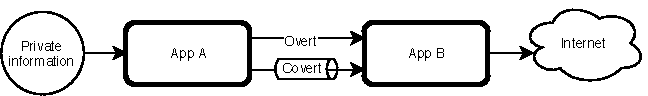
\includegraphics[width=1.0\textwidth]{figures/Collusion1}
	\caption{Structure of a basic app collusion example.}
	\label{fig:sample}
\end{figure}

An early example of this kind of collusion was described by \citeauthor{Schlegel2011}~\cite{Schlegel2011}. In their case, in place of the \app{A} was an app called Soundcomber, which obtained private information using the microphone. To avoid detection, Soundcomber did not have permission to access the internet, instead they proposed to use a second app to exfiltrate the information. A similar hypothetical example is also described by \citeauthor{Asavoae2017}~\cite{Asavoae2017}, where the \app{A} would be a contacts app with READ\_CONTACTS permission, and the \app{B} would be a weather app with INTERNET permission. However, no examples following this pattern of collusion have been reported in the real world.

There is one known example of app collusion in the wild reported by \citeauthor{Blasco2016}~\cite{Blasco2016}, and it has a different structure than described above. It is a set of apps from different vendors, all of which include a library known as the MoPlus SDK. The collusion was noticed after a manual review of apps that had already been previously categorised as potentially harmful, and were capable of accessing shared preferences files from different apps. The MoPlus SDK was already known to contain remote-control capability, and is now confirmed to also collude between different instances of itself.

The MoPlus SDK may be embedded into many different apps, with 20 such being identified by~\cite{Blasco2016}. It can then open a local HTTP server allowing the attacker to abuse any permissions given to its host app. With potentially many instances of the MoPlus SDK running on the same device with different permissions, they would work together to guarantee that only the instance with highest level of permissions is the one that starts accepting remote commands (\Fref{fig:moplus}):
\begin{enumerate}[nosep,label={(\arabic*)}]
	\item Each instance stores a priority value based on the permissions it has
	\item Each instance queries all other instances for their priorities
	\item Instance with the highest priority is called
\end{enumerate}
No sensitive information is exchanged between the apps, but still all three properties of app collusion are present.

\begin{figure}[t]
	\centering
	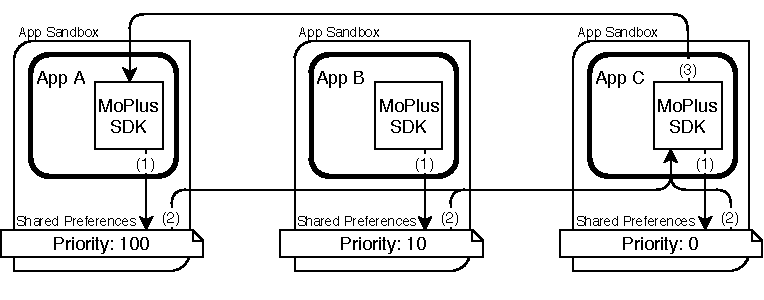
\includegraphics[width=1.0\textwidth]{figures/Collusion2}
	\caption{Collusion between instances of MoPlus SDK~\cite{Blasco2016}}
	\label{fig:moplus}
\end{figure}

\section{Existing methods for detecting collusions}
\label{sec:approaches}

Attempts with various scopes and outcomes have been made to detect app collusion. Results range from computationally feasible but very coarse filters to more accurate but very expensive approaches.

\subsection{Based on permissions/interfaces}
\label{sec:filter}

The simplest approach is to base the analysis on statically extracted features of apps, such as the set of permissions declared or the set of Android APIs imported. Only considering such features makes it feasible to scan large amounts of apps. However, the obtained results only provide a coarse estimation of app collusion.

One example by \citeauthor{Asavoae2016}~\cite{Asavoae2016} is a filtering method based on the API calls and declared permissions of apps. They define collusion as a pair of apps that satisfy these three conditions:
\begin{enumerate}[label={C\arabic*}]
	\item First app declares a permission giving access to sensitive information.
	\item Second app declares a permission giving app the ability to send information to the outside world.
	\item Finally, on some channel the first app must be able to send and second app able to receive. As channels they consider Intents (each action separately), External storage, and shared preferences (each file separately; but now deprecated as discussed in \Sref{sec:overt}).
\end{enumerate}
It is not clear from their description, but can be assumed, that they further ignore apps that match both criteria C1 and C2, since otherwise their filter would detect any pair of apps that can communicate using one of these channels. They claim that while not all apps flagged by this approach are necessarily colluding, all colluding apps are flagged by this filter. However, it must be noted that in reality they only consider a narrow subset of app collusions, and, for example, the MoPlus SDK would be labelled as benign by this filter.

\citeauthor{Chen2018}~\cite{Chen2018} propose a similar approach. First, they notice that exists a machine learning algorithm that, given the set of all API calls in an app, can predict whether the app is malicious or not. Only a single overt channel is captured for communication between apps, as their work only considers intents. For each app they detect which intents it can send and receive, and then they group together apps that could communicate with each other. To classify, whether a group of apps is benign or malicious, they pass the union of all API calls used by the apps in the group to the aforementioned machine learning algorithm.

Neither of these approaches can detect whether apps communicate with each other, nor what kind of information is exchanged between them, since they use no information about the order of operations within apps. Additionally, they both consider only a limited set of overt channels.

\subsection{Based on control flow analysis}
\label{sec:flow}

A more accurate detection of collusion can be achieved when the code of apps is analysed to detect whether or not they exchange data with other apps. Two approaches have ben taken to that: model-based and runtime.

\citeauthor{Asavoae2018}~\cite{Asavoae2018} describe a model-based method for checking whether information theft through collusion exists within the set of possible control flows for an app. They propose disassembling apps and analysing Dalvic \gls{vm} instructions with their input and output objects. In all possible control flows, when one of predefined Android APIs returns an object, it is annotated with the initiating app ID and a boolean ``sensitive''. Whenever an object is used as an argument to an instruction, its sensitivity and app ID values are propagated to all resulting objects. Input set of apps is considered to be colluding if there exists a control flow in which an object marked sensitive is passed to one of predefined exporting Android APIs, so that the current app ID is different to the initial app ID from the object. They explore modelling apps with different levels of abstraction, including more direct modelling in which case the analysis takes longer, or even forever when the app code contains any loops, and a higher level of abstraction, which is less accurate, but guaranteed to provide an answer. They only consider intent based inter-app communication channel, and do not analyse native code components of apps.

Another approach is to modify the Android \gls{os} to track information flow at runtime. \citeauthor{Enck2014} provide an example of this called TaintDroid~\cite{Enck2014}, which can track information flows from sensitive sources to sensitive sinks system wide. Within the Java code of apps it adds annotations for each variable separately (by augmenting the Java \gls{vm}), but for communication through Binder these are at message accuracy, in native system libraries with method call accuracy, and for disc access with file accuracy. TaintDroid cannot track information flow in native app components, which is solved by authors here by banning them entirely, breaking $5\%$ of apps by some estimates. Use of annotations is similar to~\cite{Asavoae2018}, but the amount of false positives is smaller, because the corresponding exit state must be reached for it to be reported. However, due to the limited granularity of annotations, their propagation can be overly conservative, which still results in false positives. False negatives are also possible, because annotations are not propagated through covert channels. Additionally, TaintDroid incurs a $14\%$ CPU overhead.

\subsection{Other}
\label{sec:othermethods}

None of the aforementioned research has adressed detection of collusion that uses covert channels. Some work has looked into closing specific covert channels~\cite{nn2017,Qi2018}, but it is not reasonable to assume that all covert channels can be found, especially since there exist known covert channels that have not been closed (\Sref{sec:covert}).

\citeauthor{Muttik2016}~\cite{Muttik2016} proposes augmenting approaches mentioned above with additional heuristic rules. He argues that colluding apps can also be detected using indirect signals, such as whether apps come from the same source, explicitly encourage co-installation, are frequently installed together, use similar libraries, etc. Furthermore, he notes that signals like publication date, app market and installation method can be used. 

According to \citeauthor{Muttik2016}, \citeauthor{McAfee2016} has a product for defending against app collusion by combining methods described in Sections \ref{sec:filter} and \ref{sec:flow}, abovementioned heuristics, and manual review and reverse engineering of apps. In 2016 \citeauthor{McAfee2016} claimed that their product is able to detect colluding mobile apps and stop any malicious combination of apps from running~\cite{McAfee2016}. However, based on known information about the state of the art, including the limitations outlined above, this is unlikely to be entirely true.

\section{Conclusion}
\label{sec:conclusion}

This report presented an overview of Android app collusion. It surveyed state-of-the-art literature discussing methods that can be used for collusion on Android, and known examples of such collusion. This report also discussed existing approaches to app collusion detection, and their limitations.

The number and complexity of malware attacks against Android are increasing, which is especially concerning because mobile devices are rich sources of data. One of the threats that cannot yet be reliably detected nor defended against is app collusion, which can be defined as a secret collaboration between apps with malicious intentions. The Android \gls{os} has multiple overt and covert channels for apps to exploit for colluding. However, some communication channels that had been described by researchers, such as the ones based on \texttt{/proc/stat} or shared preferences, were determined to no longer be relevant due to changes in Android. An interesting future work would be to reproduce covert channels used for collusion, in order to confirm, which channels are still exploitable.

Existing literature on app collusion detection was also determined to have significant limitations. Multiple proposed solutions used some definition of app collusion that did not differenciate collusion from legitimate collaboration, or only included a subset of collusions, e.g., information exfiltration, making these definitions not applicable in the real world. One source has also made what seems to be an uncredible claim of having solved the problem of app collusion. 

From the literature it is clear that further research is required to develop feasible protections against Android app collusion. This report provided a comparison of the proposed collusion methods and protections using a common definition and criteria. These definitions and criteria could be further developed into a common framework, and could assist the research community in achieveving results in the detection of app collusion.

%============================================================

\bibliographystyle{IEEEtranNDoi}
\bibliography{ieee,oro-cs-seminar}

\end{document}
